% Contributions are much appreciated, in order to contribute to this project, head over to this repository:
% https://github.com/bshramin/uofa-eng-assignment

\documentclass[11pt,letterpaper]{article}
\textwidth 6.5in
\textheight 9.in
\oddsidemargin 0in
\headheight 0in
\usepackage{graphicx}
\usepackage{fancybox}
\usepackage[utf8]{inputenc}
\usepackage{epsfig,graphicx}
\usepackage{multicol,pst-plot}
\usepackage{pstricks}
\usepackage{amsmath}
\usepackage{amsfonts}
\usepackage{amssymb}
\usepackage{eucal}
\usepackage[left=2cm,right=2cm,top=2cm,bottom=2cm]{geometry}
\usepackage{esvect}
\pagestyle{empty}
\DeclareMathOperator{\tr}{Tr}
\newcommand*{\op}[1]{\check{\mathbf#1}}
\newcommand{\bra}[1]{\langle #1 |}
\newcommand{\ket}[1]{| #1 \rangle}
\newcommand{\braket}[2]{\langle #1 | #2 \rangle}
\newcommand{\mean}[1]{\langle #1 \rangle}
\newcommand{\opvec}[1]{\check{\vec #1}}
\renewcommand{\sp}[1]{$${\begin{split}#1\end{split}}$$}

\usepackage{lipsum}

\usepackage{listings}
\usepackage{color}
\usepackage{wrapfig}
\usepackage[shortlabels]{enumitem}

\definecolor{codegreen}{rgb}{0,0.6,0}
\definecolor{codegray}{rgb}{0.5,0.5,0.5}
\definecolor{codepurple}{rgb}{0.58,0,0.82}
\definecolor{backcolour}{rgb}{0.95,0.95,0.92}

\lstdefinestyle{mystyle}{
	backgroundcolor=\color{backcolour},   
	commentstyle=\color{codegreen},
	keywordstyle=\color{magenta},
	numberstyle=\tiny\color{codegray},
	stringstyle=\color{codepurple},
	basicstyle=\footnotesize,
	breakatwhitespace=false,         
	breaklines=true,                 
	captionpos=b,                    
	keepspaces=true,                 
	numbers=left,                    
	numbersep=5pt,                  
	showspaces=false,                
	showstringspaces=false,
	showtabs=false,                  
	tabsize=2
}

\lstset{style=mystyle}

\begin{document}
\pagestyle{plain}

\begin{flushleft}
Estudiante: Fabio Quimbay\\
Email: fabio.quimbay883@comunidadunir.net\\
Profesor: Miguel Ángel Cabeza\\
Fecha: Noviembre 14 de 2022\\
\end{flushleft}

\begin{flushright}\vspace{-20mm}

\includegraphics[height=2cm]{logo.png}
\end{flushright}
 
\begin{center}\vspace{0cm}
\textbf{\large PER5786 2022-2023  Física 1 (GFI) - PER5786 2022-2023}\\
 Tema 3 - Movimientos elementales
\end{center}

 
\rule{\linewidth}{0.1mm}
%%%%%%%%%%%%%%%%%%%%%%%%%%%%%%%%%%%%%%%%%%%%%%%%%%%%%%%%%%%%%%%%%%%%%%%%

\bigskip
\bigskip

%%%%%%%%%%%%%%%%%%%%
\textbf{Problema propuesto 8}\\

Un "volante de inercia" (flywheel) del sistema KERS de recuperación de energía en frenada para un vehículo de Fórmula 1, es capaz de girar a 64,500 rpm con un radio de 24 cm en tan solo 3 segundos partiendo de reposo. Calcula su aceleración angular, y la velocidad a los 2 segundos.

\begin{wrapfigure}{r}{0.25\textwidth}
\begin{center}
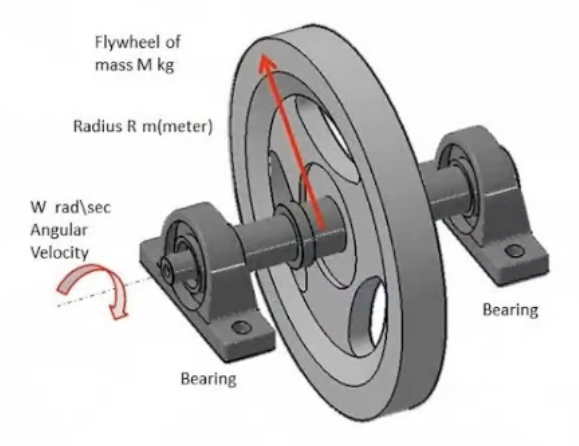
\includegraphics[width=0.25\textwidth]{problema_8.png}
\end{center}
\end{wrapfigure}

\textbf{Formulas base:}\\

Se tomarán las siguientes formulas base del MCUA:

\begin{align}
\boxed{ \omega = \omega_{0} + \alpha \cdot (t - t_{0})} \Rightarrow
\boxed{ \alpha = \frac{\omega - \omega_{0}}{t - t_{0}}}\\
\boxed{ \theta = \theta_{0} + \omega_{0} \cdot (t - t_{0}) + \frac{1}{2} \cdot \alpha \cdot (t - t_{0})}
\end{align}

\textbf{Solución:}\\

Primero es necesario establecer todos los parámetros en términos de las unidades del SI, a saber:

\begin{align}
\omega = \frac{64500\,vueltas}{1\,min} = \frac{2 \cdot \pi \cdot 64500\,rad}{60\,s} = 2150 \cdot \pi = 6754.42\,rad/s
\end{align}

Ahora se calcula la aceleración angular durante el todo el recorrido dado, durante los 3 segundos, así:

\begin{align}
\alpha_{t=3} = \frac{\omega}{t} = \frac{6754.42}{3} = 2251.47\,rad/s^2
\end{align}

Con el valor de $\alpha$ calculado, ahora podemos establecer la velocidad angular y velocidad en $t=2\,s$ a saber:

\begin{align}
\omega_{t=2} = 0 + 2251.47 \cdot (2) = 4502.95\,rad/s^2\\
V_{t=2} = \omega \cdot r = 4502.95 \cdot 0.24 = 1080.71\,m/s 
\end{align}

La aceleración angular y velocidad en $t = 2\,s$ son $4502.95\,rad/s^2$ y $1080.71\,m/s$, respectivamente.

%%%%%%%%%%%%%%%%%%%%

\end{document}

